\documentclass[10pt, aspectratio=169]{beamer}
\usetheme{metropolis}

% Dark theme configuration
\definecolor{bgdark}{HTML}{06080D}
\definecolor{bgcard}{HTML}{111620}
\definecolor{fgwhite}{HTML}{FFFFFF}
\definecolor{fggray}{HTML}{8B95A5}
\definecolor{accentcyan}{HTML}{22D3EE}
\definecolor{accentpurple}{HTML}{A78BFA}
\definecolor{accentblue}{HTML}{4DA8FF}
\definecolor{accentgreen}{HTML}{10B981}
\definecolor{accentorange}{HTML}{F97316}
\definecolor{accentred}{HTML}{EC111A}
\definecolor{accentyellow}{HTML}{F59E0B}

\setbeamercolor{normal text}{fg=fgwhite, bg=bgdark}
\setbeamercolor{alerted text}{fg=accentcyan}
\setbeamercolor{frametitle}{fg=fgwhite, bg=bgcard}
\setbeamercolor{title}{fg=fgwhite}
\setbeamercolor{subtitle}{fg=fggray}
\setbeamercolor{author}{fg=fggray}
\setbeamercolor{date}{fg=fggray}
\setbeamercolor{institute}{fg=fggray}
\setbeamercolor{block title}{fg=bgdark, bg=accentcyan}
\setbeamercolor{block body}{fg=fgwhite, bg=bgcard}
\setbeamercolor{block title alerted}{fg=bgdark, bg=accentred}
\setbeamercolor{block body alerted}{fg=fgwhite, bg=bgcard}
\setbeamercolor{block title example}{fg=bgdark, bg=accentgreen}
\setbeamercolor{block body example}{fg=fgwhite, bg=bgcard}
\setbeamercolor{itemize item}{fg=accentcyan}
\setbeamercolor{itemize subitem}{fg=accentpurple}
\setbeamercolor{enumerate item}{fg=accentcyan}
\setbeamercolor{section in toc}{fg=fgwhite}
\setbeamercolor{progress bar}{fg=accentcyan, bg=bgcard}
\setbeamercolor{footnote}{fg=fggray}

\setbeamertemplate{navigation symbols}{}
\setbeamertemplate{footline}{
  \hfill\usebeamerfont{footline}\usebeamercolor[fg]{footline}
  \insertframenumber/\inserttotalframenumber\hspace*{0.5em}\vspace{0.3em}
}
\setbeamercolor{footline}{fg=fggray}

% Packages
\usepackage{amsmath, amssymb}
\usepackage{booktabs}
\usepackage{tikz}
\usetikzlibrary{shapes.geometric, arrows.meta, positioning, calc, fit, decorations.pathreplacing}
\usepackage{listings}
\usepackage{xcolor}

\lstset{
  basicstyle=\ttfamily\scriptsize\color{fgwhite},
  backgroundcolor=\color{bgcard},
  keywordstyle=\color{accentpurple},
  commentstyle=\color{fggray}\itshape,
  stringstyle=\color{accentgreen},
  frame=none,
  breaklines=true,
  showstringspaces=false,
}

% Custom commands
\newcommand{\cmark}{\textcolor{accentgreen}{\checkmark}}
\newcommand{\xmark}{\textcolor{accentred}{\texttimes}}
\newcommand{\hlt}[1]{\textcolor{accentcyan}{#1}}
\newcommand{\hlp}[1]{\textcolor{accentpurple}{#1}}
\newcommand{\hlg}[1]{\textcolor{accentgreen}{#1}}
\newcommand{\hlo}[1]{\textcolor{accentorange}{#1}}
\newcommand{\hlr}[1]{\textcolor{accentred}{#1}}

% Title info
\title{S2A Platform: Signal-to-Action}
\subtitle{An Agentic LLM Architecture for\\Automated AML Feature Engineering}
\author{Jerry Li}
\institute{AML Research Team \(\cdot\) Scotiabank}
\date{March 2026}

\begin{document}

% ============================================================
% SLIDE 1: TITLE
% ============================================================
\begin{frame}[plain]
  \maketitle
  \vspace{-1.5em}
  \begin{center}
    \colorbox{bgcard}{%
      \parbox{0.85\textwidth}{\centering\small\ttfamily\color{accentcyan}%
        Regulatory Text \(\to\) 6 AI Agents \(\to\) Executable Features \(\to\) Anomaly Detection \(\to\) Regulatory Verification%
      }%
    }
  \end{center}
\end{frame}

% ============================================================
% SLIDE 2: PROBLEM
% ============================================================
\begin{frame}{Current Operating Model: The Feature Engineering Bottleneck}

\begin{columns}[T]
\begin{column}{0.48\textwidth}
  \textbf{AML Typology Model Development}
  \vspace{0.5em}

  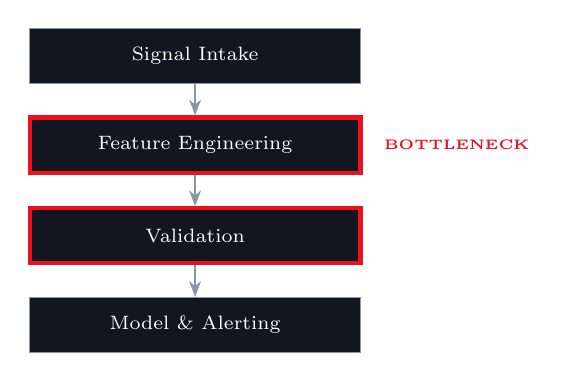
\begin{tikzpicture}[
    node distance=0.4cm,
    box/.style={rectangle, draw=fggray, fill=bgcard, text=fgwhite, minimum width=4.2cm, minimum height=0.7cm, align=center, font=\scriptsize},
    bottleneck/.style={rectangle, draw=accentred, fill=bgcard, text=fgwhite, minimum width=4.2cm, minimum height=0.7cm, align=center, font=\scriptsize, line width=1.5pt},
    arr/.style={-{Stealth[length=2mm]}, fggray, thick},
  ]
    \node[box] (s1) {Signal Intake};
    \node[bottleneck, below=of s1] (s2) {Feature Engineering};
    \node[bottleneck, below=of s2] (s3) {Validation};
    \node[box, below=of s3] (s4) {Model \& Alerting};

    \draw[arr] (s1) -- (s2);
    \draw[arr] (s2) -- (s3);
    \draw[arr] (s3) -- (s4);

    \node[right=0.15cm of s2, font=\tiny\bfseries, text=accentred] {\rotatebox{0}{BOTTLENECK}};
  \end{tikzpicture}
\end{column}

\begin{column}{0.50\textwidth}
  \textbf{\hlr{Key Pain Points}}
  \vspace{0.3em}

  \begin{itemize}\itemsep0.5em
    \item[\hlr{\textbullet}] \small Analyst manually reads and interprets regulatory documents --- slow, subjective, and inconsistent across analysts
    \item[\hlr{\textbullet}] \small Feature design tied to individual expertise; knowledge lost when the analyst leaves, similar typologies rebuilt from scratch
    \item[\hlr{\textbullet}] \small Validation only at model fitting stage --- errors caught too late in the development cycle
    \item[\hlr{\textbullet}] \small No traceability from feature back to regulatory source --- audit gaps
  \end{itemize}
\end{column}
\end{columns}
\end{frame}

% ============================================================
% SLIDE 3: ARCHITECTURE OVERVIEW
% ============================================================
\begin{frame}{System Architecture: 6-Agent Pipeline}

\begin{center}
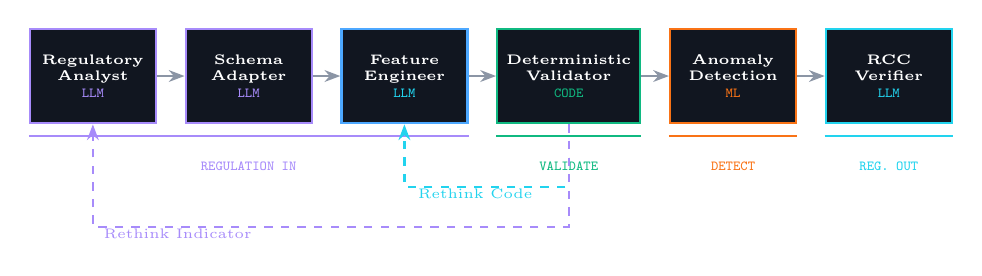
\begin{tikzpicture}[
  node distance=0.2cm,
  agent/.style={rectangle, draw=#1, fill=bgcard, text=fgwhite, minimum width=1.6cm, minimum height=1.2cm, align=center, font=\tiny, line width=0.8pt},
  arr/.style={-{Stealth[length=2mm]}, fggray, thick},
  label/.style={font=\tiny\bfseries, text=#1},
  phase/.style={font=\tiny\ttfamily, text=#1},
]
  % Agents
  \node[agent=accentpurple] (a1) {\textbf{Regulatory}\\\textbf{Analyst}\\\hlp{\texttt{LLM}}};
  \node[agent=accentpurple, right=0.35cm of a1] (a2) {\textbf{Schema}\\\textbf{Adapter}\\\hlp{\texttt{LLM}}};
  \node[agent=accentblue, right=0.35cm of a2] (a3) {\textbf{Feature}\\\textbf{Engineer}\\\hlt{\texttt{LLM}}};
  \node[agent=accentgreen, right=0.35cm of a3] (a4) {\textbf{Deterministic}\\\textbf{Validator}\\\hlg{\texttt{CODE}}};
  \node[agent=accentorange, right=0.35cm of a4] (a5) {\textbf{Anomaly}\\\textbf{Detection}\\\hlo{\texttt{ML}}};
  \node[agent=accentcyan, right=0.35cm of a5] (a6) {\textbf{RCC}\\\textbf{Verifier}\\\hlt{\texttt{LLM}}};

  \draw[arr] (a1) -- (a2);
  \draw[arr] (a2) -- (a3);
  \draw[arr] (a3) -- (a4);
  \draw[arr] (a4) -- (a5);
  \draw[arr] (a5) -- (a6);

  % Phase labels
  \node[phase=accentpurple, below=0.35cm of a2] (p1) {REGULATION IN};
  \draw[accentpurple, thick] (a1.south west) ++(0,-0.15) -- ($(a3.south east)+(0,-0.15)$);

  \node[phase=accentgreen, below=0.35cm of a4] {VALIDATE};
  \draw[accentgreen, thick] (a4.south west) ++(0,-0.15) -- ($(a4.south east)+(0,-0.15)$);

  \node[phase=accentorange, below=0.35cm of a5] {DETECT};
  \draw[accentorange, thick] (a5.south west) ++(0,-0.15) -- ($(a5.south east)+(0,-0.15)$);

  \node[phase=accentcyan, below=0.35cm of a6] {REG.\ OUT};
  \draw[accentcyan, thick] (a6.south west) ++(0,-0.15) -- ($(a6.south east)+(0,-0.15)$);

  % Self-correction loop: Validator → Engineer (code-level fix)
  \draw[accentcyan, dashed, thick, -{Stealth[length=2mm]}] (a4.south) -- ++(0,-0.8) -| (a3.south);
  \node[font=\tiny, text=accentcyan, below=0.7cm of a3, xshift=0.9cm] {Rethink Code};

  % Rethink loop: Validator → Analyst (indicator-level rethink)
  \draw[accentpurple, dashed, thick, -{Stealth[length=2mm]}] (a4.south) -- ++(0,-1.3) -| (a1.south);
  \node[font=\tiny, text=accentpurple, below=1.2cm of a2, xshift=-0.9cm] {Rethink Indicator};
\end{tikzpicture}
\end{center}

\vspace{0.3em}

\begin{columns}[T]
\begin{column}{0.32\textwidth}
  \begin{block}{Perceive--Reason--Act}
    \scriptsize Each agent produces structured, auditable output at every step following the PRA loop.
  \end{block}
\end{column}
\begin{column}{0.32\textwidth}
  \begin{block}{Neuro-Symbolic Detection}
    \scriptsize Symbolic (regulation) + Neural (LLM compilation) + Statistical (Isolation Forest).
  \end{block}
\end{column}
\begin{column}{0.32\textwidth}
  \begin{block}{Closed-Loop Grounding}
    \scriptsize Same regulatory text used for feature compilation AND alert verification.
  \end{block}
\end{column}
\end{columns}
\end{frame}

% ============================================================
% SLIDE 4: REGULATION IN — Agents 1–3
% ============================================================
\begin{frame}{Regulation In: Agents 1--3}

\begin{columns}[T]
\begin{column}{0.32\textwidth}
  \textbf{\hlp{Agent 1: Regulatory Analyst}} {\tiny\texttt{GPT-4o}}
  \vspace{0.3em}

  \scriptsize
  \textbf{Input:} Raw regulatory text\\[0.3em]
  \textbf{Output:}
  \begin{itemize}\itemsep0.15em
    \item \textbf{Indicator:} category (from 20-type ontology), description, risk rationale
    \item \textbf{Parameters:} thresholds with regulatory basis (e.g.\ \$10K CTR limit)
    \item \textbf{Computation plan:} operation, time window, required columns
  \end{itemize}
\end{column}

\begin{column}{0.32\textwidth}
  \textbf{\hlp{Agent 2: Schema Adapter}} {\tiny\texttt{GPT-4o}}
  \vspace{0.3em}

  \scriptsize
  \textbf{Input:} Indicator + target schema\\[0.3em]
  \textbf{Output:} Per-channel compatibility:
  \begin{itemize}\itemsep0.15em
    \item \hlg{\texttt{direct\_match}} --- column exists
    \item \hlo{\texttt{proxy\_required}} --- substitute available
    \item \hlr{\texttt{not\_feasible}} --- cannot compute
  \end{itemize}

  \vspace{0.3em}
  Same regulation \(\to\) different code per schema.
\end{column}

\begin{column}{0.32\textwidth}
  \textbf{\hlt{Agent 3: Feature Engineer}} {\tiny\texttt{GPT-4o}}
  \vspace{0.3em}

  \scriptsize
  \textbf{Input:} Indicator + schema mapping\\[0.3em]
  \textbf{Output:}
  \begin{itemize}\itemsep0.15em
    \item Python function:\\
      \texttt{compute\_feature(df, accounts\_df)}
    \item PRA comments embedded in code (regulatory provenance)
  \end{itemize}

  \vspace{0.3em}
  Code is grounded in regulatory reasoning at every step.
\end{column}
\end{columns}

\end{frame}

% ============================================================
% SLIDE 5: VALIDATION — Agent 4
% ============================================================
\begin{frame}{Deterministic Validation: Agent 4}

\textbf{\hlg{Agent 4}} is \textit{not} an LLM --- it is a deterministic code validator with three verification stages:

\vspace{0.5em}
\begin{columns}[T]
\begin{column}{0.32\textwidth}
  \begin{exampleblock}{1. AST Safety}
    \scriptsize
    Static analysis of generated code:
    \begin{itemize}\itemsep0.15em
      \item Banned imports: \texttt{os}, \texttt{sys}, \texttt{subprocess}
      \item Banned calls: \texttt{eval}, \texttt{exec}, \texttt{open}
      \item No file I/O or network access
    \end{itemize}
  \end{exampleblock}
\end{column}

\begin{column}{0.32\textwidth}
  \begin{exampleblock}{2. Column Alignment}
    \scriptsize
    Every column the code reads must exist in the target schema.
    \begin{itemize}\itemsep0.15em
      \item Extracts column refs via AST
      \item On mismatch: \textit{Find Similar} / \textit{Rethink} / \textit{Skip}
    \end{itemize}
  \end{exampleblock}
\end{column}

\begin{column}{0.32\textwidth}
  \begin{exampleblock}{3. Statistical Validation}
    \scriptsize
    Feature quality metrics:
    \begin{itemize}\itemsep0.15em
      \item \textbf{KS Statistic} (distribution divergence)
      \item \textbf{Information Value} (predictive power)
    \end{itemize}
    If IV \(< 0.02\): triggers diagnostic feedback loop.
  \end{exampleblock}
\end{column}
\end{columns}

\vspace{0.5em}
\textbf{Feedback Loops} (up to 5 iterations each):
\[
  \text{Validator} \xrightarrow[\text{\tiny Rethink Code}]{\text{error}} \text{Engineer} \xrightarrow{\text{fix}} \text{Validator}
  \qquad\qquad
  \text{Validator} \xrightarrow[\text{\tiny Rethink Indicator}]{\text{low IV}} \text{Analyst} \xrightarrow{\text{new indicator}} \text{Validator}
\]
If convergence fails \(\to\) \hlt{Human-in-the-Loop} decision: Rethink Indicator / Rethink Code / Continue with Benchmarks / Stop.
\end{frame}

% ============================================================
% SLIDE 6: STATISTICAL METRICS
% ============================================================
\begin{frame}{Statistical Validation Metrics}

\begin{columns}[T]
\begin{column}{0.48\textwidth}
  \begin{block}{Information Value (IV)}
    \scriptsize
    Measures feature's discriminatory power between positive (suspicious) and negative (normal) populations:
    \[
      \text{IV} = \sum_{i=1}^{B} \left(\frac{e_i}{E} - \frac{n_i}{N}\right) \cdot \ln\!\left(\frac{e_i / E}{n_i / N}\right)
    \]
    where \(e_i, n_i\) = events/non-events in bin \(i\), and \(E = \sum e_i,\; N = \sum n_i\).

    \vspace{0.5em}
    \begin{tabular}{ll}
      \toprule
      \textbf{IV Range} & \textbf{Interpretation} \\
      \midrule
      \(< 0.02\) & Not predictive \(\to\) \hlr{triggers feedback} \\
      \(0.02 - 0.1\) & Weak \\
      \(0.1 - 0.3\) & Medium \\
      \(0.3 - 0.5\) & Strong \\
      \(> 0.5\) & Very strong (check overfit) \\
      \bottomrule
    \end{tabular}
  \end{block}
\end{column}

\begin{column}{0.48\textwidth}
  \begin{block}{Kolmogorov--Smirnov (KS) Statistic}
    \scriptsize
    Maximum distance between CDFs of positive and negative groups:
    \[
      D_{KS} = \sup_x \left| F_{\text{pos}}(x) - F_{\text{neg}}(x) \right|
    \]

    \begin{itemize}\itemsep0.2em
      \item \(D_{KS} = 0\): identical distributions
      \item \(D_{KS} = 1\): perfect separation
      \item Used alongside IV for robust quality assessment
    \end{itemize}
  \end{block}

  \vspace{0.3em}
  \begin{block}{Decision Threshold}
    \scriptsize
    When IV \(< 0.02\), the \hlt{Diagnostic Agent} analyzes root cause:
    \begin{itemize}\itemsep0.1em
      \item Feature semantically valid but data insufficient?
      \item Computation approach suboptimal?
      \item Indicator not applicable to this schema?
    \end{itemize}
    Options narrow after each retry (tried options removed).
  \end{block}
\end{column}
\end{columns}
\end{frame}

% ============================================================
% SLIDE 7: DETECTION & RCC
% ============================================================
\begin{frame}{Anomaly Detection (Agent 5) \& RCC Verification (Agent 6)}

\begin{columns}[T]
\begin{column}{0.48\textwidth}
  \textbf{\hlo{Agent 5: Isolation Forest}} {\scriptsize (Liu et al., 2008)}
  \vspace{0.3em}

  \scriptsize
  Key insight: anomalies are \textit{few and different} --- require fewer random splits to isolate.

  \vspace{0.3em}
  \textbf{Anomaly score} for instance \(x\):
  \[
    s(x, n) = 2^{-\frac{E[h(x)]}{c(n)}}
  \]
  where \(h(x)\) = path length, \(c(n)\) = average path length in unsuccessful BST search.

  \vspace{0.3em}
  \begin{tabular}{ll}
    \toprule
    \textbf{Parameter} & \textbf{Value} \\
    \midrule
    Features & 10 benchmark + \(N\) compiled \\
    Split & 70/30 stratified \\
    Flagging & Top-15 accounts by score \\
    Contamination & From empirical positive rate \\
    \bottomrule
  \end{tabular}

  \vspace{0.3em}
  \textbf{Evaluation:} AUC-ROC, Precision@K, Recall@K, F1

  Labels used \textit{only} for evaluation, not training.
\end{column}

\begin{column}{0.48\textwidth}
  \textbf{\hlt{Agent 6: RCC Verifier}} --- \textit{``Regulation Out''}
  \vspace{0.3em}

  \scriptsize
  Closes the loop: verifies each alert against the \textit{same} regulatory text that compiled the feature.

  \vspace{0.3em}
  \textbf{Input:} Flagged customer's feature values + source regulation

  \textbf{Output:} Structured verdict per alert:
  \begin{itemize}\itemsep0.2em
    \item \textbf{Verdict:} \hlg{\texttt{supported}} / \hlr{\texttt{contradicted}} / \hlo{\texttt{ambiguous}}
    \item \textbf{Confidence:} high / medium / low
    \item \textbf{Evidence cards:} feature value vs.\ population mean, regulatory criterion, quoted regulatory text
  \end{itemize}

  \vspace{0.3em}
\end{column}
\end{columns}

\vspace{0.2em}
\begin{block}{Closed-Loop Grounding}
  \scriptsize
  \textbf{Regulation In:} text \(\xrightarrow{\text{compile}}\) feature \hfill
  \textbf{Regulation Out:} alert \(\xrightarrow{\text{verify}}\) same text \hfill
  Audit-traceable end-to-end.
\end{block}
\end{frame}

% ============================================================
% SLIDE 7b: RFS — What the Pipeline Produces
% ============================================================
\begin{frame}{Regulatory Feature Specification (RFS)}

\vspace{-0.3em}
\begin{center}
\scriptsize\color{fggray} The pipeline is the factory. The RFS is the \textbf{product} --- a complete, traceable, reusable feature package.
\end{center}

\vspace{0.2em}
\begin{center}
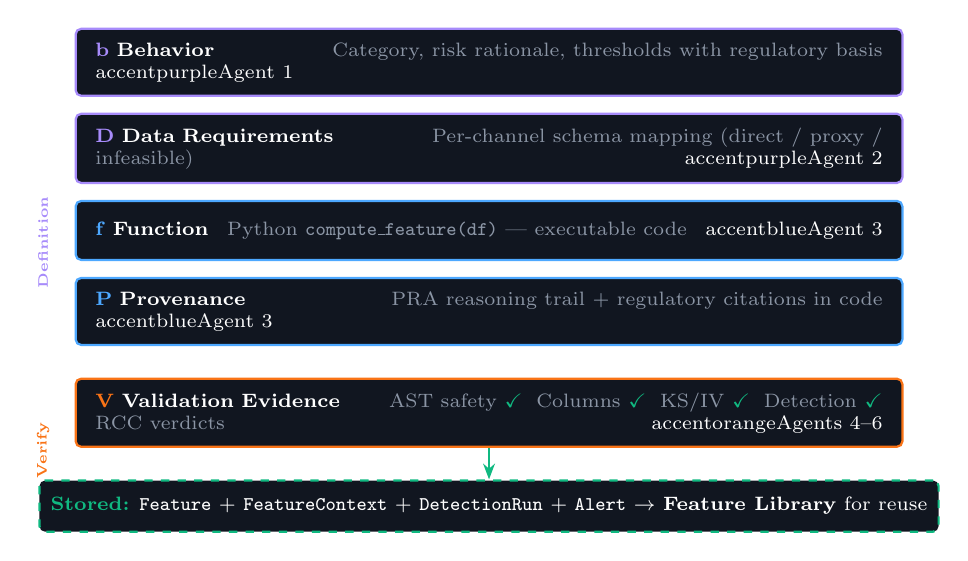
\begin{tikzpicture}[
  node distance=0.2cm,
  row/.style={rectangle, draw=#1, fill=bgcard, text=fgwhite,
    minimum width=10.5cm, minimum height=0.75cm,
    align=left, font=\scriptsize, line width=0.8pt, rounded corners=2pt,
    text width=10cm, inner sep=5pt},
  agl/.style={font=\tiny\bfseries, text=#1},
  db/.style={rectangle, draw=accentgreen, fill=bgcard, text=fgwhite,
    minimum width=10.5cm, minimum height=0.65cm,
    align=center, font=\scriptsize, line width=0.8pt, rounded corners=2pt, dashed,
    inner sep=4pt},
]
  % --- Definition rows (Agents 1-3) ---
  \node[row=accentpurple] (b) {%
    \textcolor{accentpurple}{\textbf{b}} \textbf{Behavior}%
    \hfill {\color{fggray}Category, risk rationale, thresholds with regulatory basis}%
    \hfill {\agl{accentpurple}Agent 1}%
  };
  \node[row=accentpurple, below=of b] (d) {%
    \textcolor{accentpurple}{\textbf{D}} \textbf{Data Requirements}%
    \hfill {\color{fggray}Per-channel schema mapping (direct / proxy / infeasible)}%
    \hfill {\agl{accentpurple}Agent 2}%
  };
  \node[row=accentblue, below=of d] (f) {%
    \textcolor{accentblue}{\textbf{f}} \textbf{Function}%
    \hfill {\color{fggray}Python \texttt{compute\_feature(df)} --- executable code}%
    \hfill {\agl{accentblue}Agent 3}%
  };
  \node[row=accentblue, below=of f] (p) {%
    \textcolor{accentblue}{\textbf{P}} \textbf{Provenance}%
    \hfill {\color{fggray}PRA reasoning trail + regulatory citations in code}%
    \hfill {\agl{accentblue}Agent 3}%
  };

  % --- Validation row (Agents 4-6) ---
  \node[row=accentorange, below=0.4cm of p] (v) {%
    \textcolor{accentorange}{\textbf{V}} \textbf{Validation Evidence}%
    \hfill {\color{fggray}AST safety \cmark\; Columns \cmark\; KS/IV \cmark\; Detection \cmark\; RCC verdicts}%
    \hfill {\agl{accentorange}Agents 4--6}%
  };

  % --- Bracket labels ---
  \node[left=0.4cm of $(b.north west)!0.5!(p.south west)$, font=\tiny\bfseries, text=accentpurple, align=center, rotate=90] {Definition};
  \node[left=0.4cm of v.west, font=\tiny\bfseries, text=accentorange, align=center, rotate=90] {Verify};

  % --- DB row ---
  \node[db, below=0.4cm of v] (db) {%
    \textcolor{accentgreen}{\textbf{Stored:}} \texttt{Feature} + \texttt{FeatureContext} + \texttt{DetectionRun} + \texttt{Alert} \(\to\) \textbf{Feature Library} for reuse%
  };
  \draw[accentgreen, thick, -{Stealth[length=2mm]}] (v.south) -- (db.north);
\end{tikzpicture}
\end{center}

\vspace{0.2em}
\begin{columns}[T]
\begin{column}{0.48\textwidth}
  \begin{block}{Knowledge Preservation}
    \scriptsize A good feature is never lost. Promote to library for reuse across future typologies.
  \end{block}
\end{column}
\begin{column}{0.48\textwidth}
  \begin{block}{Audit Trail}
    \scriptsize Every feature \(\to\) regulatory source. Every alert \(\to\) feature. End-to-end provenance.
  \end{block}
\end{column}
\end{columns}
\end{frame}

% ============================================================
% SLIDE 8: WHY NOT SINGLE-PASS
% ============================================================
\begin{frame}{Why Multi-Agent? Comparison with Single-Pass Approaches}

\begin{center}
\scriptsize
\begin{tabular}{p{4.2cm}ccc}
  \toprule
  \textbf{Property} & \textbf{Single-Pass LLM} & \textbf{Prompt Eng.} & \textbf{Multi-Agent (Ours)} \\
  \midrule
  Independent validation & \xmark & \xmark & \cmark \\
  Output consistency across runs & \xmark & \xmark & \cmark\;(deterministic validator) \\
  Pinpointed failure diagnosis & \xmark & \xmark & \cmark\;(per-agent error trace) \\
  Self-correction loop & \xmark & \xmark & \cmark\;(Validator $\leftrightarrow$ Engineer) \\
  Regulatory traceability & \xmark & \xmark & \cmark\;(provenance in RFS) \\
  Separated context windows & \xmark & \xmark & \cmark\;(no attention dilution) \\
  Schema-adaptive compilation & \xmark & \xmark & \cmark\;(Adapter agent) \\
  Audit-ready output & \xmark & \xmark & \cmark\;(PRA at every step) \\
  \bottomrule
\end{tabular}
\end{center}

\vspace{0.5em}
\begin{alertblock}{Key Insight}
  \small The value is not \textit{generation} --- it is \textbf{validated, auditable generation with self-correction}. A single LLM call cannot independently verify its own output; separated agents with deterministic boundaries can.
\end{alertblock}
\end{frame}

% ============================================================
% SLIDE 9: DATASET & RESULTS
% ============================================================
\begin{frame}{Dataset \& Results}

\begin{columns}[T]
\begin{column}{0.45\textwidth}
  \textbf{IBM AML HI-Small} {\scriptsize (primary benchmark)}
  \vspace{0.3em}

  \scriptsize
  \begin{tabular}{ll}
    \toprule
    Transactions & 5,078,415 \\
    Unique accounts & 496,995 \\
    Positive accounts & 3,376 (0.68\%) \\
    Source & IBM AMLSim (Kaggle) \\
    \bottomrule
  \end{tabular}

  \vspace{0.3em}
  {\tiny Demo uses a stratified subsample for speed; full dataset available for batch evaluation.}

  \vspace{0.5em}
  \textbf{FINTRAC} {\scriptsize (schema adaptation demo)}
  \vspace{0.3em}

  \scriptsize 7 channels: Card (3.5M), EFT (1.1M), EMT (846K), Cheque (241K), ABM (186K), Wire (5K), WU (2K).

  Demonstrates multi-channel schema-adaptive compilation.

  \vspace{0.5em}
  \textbf{10 Benchmark Features} {\scriptsize (domain-agnostic)}

  \scriptsize Statistical baselines requiring no regulatory knowledge: \texttt{total\_amount}, \texttt{txn\_count}, \texttt{amount\_std}, \texttt{unique\_counterparties}, \texttt{temporal\_spread}, \texttt{non\_self\_transfer\_ratio}, \texttt{ach\_ratio}, \texttt{foreign\_txn\_ratio}, \texttt{median\_amount}, \texttt{payment\_diversity}.
\end{column}

\begin{column}{0.50\textwidth}
  \textbf{Key Results}
  \vspace{0.3em}

  \scriptsize
  The core question: does a regulation-compiled feature add detection value on top of domain-agnostic statistical baselines?

  \vspace{0.3em}
  \begin{center}
  \scriptsize
  \begin{tabular}{lcc}
    \toprule
    \textbf{Configuration} & \textbf{AUC-ROC} & \textbf{Features} \\
    \midrule
    10 benchmark only & baseline & 10 \\
    10 benchmark + compiled & baseline + \(\Delta\) & 11 \\
    \bottomrule
  \end{tabular}
  \end{center}

  \vspace{0.3em}
  \scriptsize
  The \(\Delta\) demonstrates the marginal detection gain from a \textit{single} regulation-compiled feature. Results shown in live demo.

  \vspace{0.5em}
  \begin{block}{Pipeline Performance}
    \scriptsize
    \begin{tabular}{ll}
      Compilation time & $\sim$2--3 min (vs.\ days manual) \\
      Self-correction & Up to 5 auto-iterations \\
      Traceability & RCC maps every alert to regulation \\
      Schema portability & FINTRAC vs.\ IBM AML verified \\
    \end{tabular}
  \end{block}
\end{column}
\end{columns}
\end{frame}

% ============================================================
% SLIDE 10: DEMO & NEXT STEPS
% ============================================================
\begin{frame}{Live Demo \& Next Steps}

\begin{columns}[T]
\begin{column}{0.48\textwidth}
  \textbf{Demo: Two Runs}
  \vspace{0.3em}

  \begin{alertblock}{Run 1: Self-Correction}
    \scriptsize
    ``Iran is a high-risk country'' \(\to\) Analyst extracts \texttt{geographic\_risk} \(\to\) Engineer generates code \(\to\) Validator: AST pass but IV\(=0\) \(\to\) Diagnostic Agent analyzes root cause \(\to\) Human decision: Rethink Indicator / Rethink Code / Continue with Benchmarks \(\to\) Graceful fallback.

    \vspace{0.3em}
    \textit{Story: ``System tries, diagnoses failures, and falls back gracefully.''}
  \end{alertblock}

  \vspace{0.3em}
  \begin{exampleblock}{Run 2: Full Pipeline}
    \scriptsize
    FINTRAC operational alert \(\to\) 6 agents \(\to\) compiled feature passes validation \(\to\) Isolation Forest detection \(\to\) RCC verdict + evidence cards.

    \vspace{0.3em}
    \textit{Story: ``Regulation In \(\to\) Detection \(\to\) Regulation Out. Full traceability.''}
  \end{exampleblock}
\end{column}

\begin{column}{0.48\textwidth}
  \textbf{Research Directions}
  \vspace{0.3em}

  \scriptsize
  \begin{enumerate}\itemsep0.5em
    \item \textbf{Feature Quality Benchmarking} {\tiny\hlg{In Progress}}\\
      Systematic comparison: S2F-compiled vs.\ single-pass GPT vs.\ human-designed. Correctness, detection utility, coverage.

    \item \textbf{Self-Correction Pattern Research} {\tiny\hlo{Planned}}\\
      Failure rates by indicator category, common error types, convergence speed. Error taxonomy.

    \item \textbf{Typology Coverage Intelligence} {\tiny\hlo{Planned}}\\
      Feature landscape across all FINTRAC typologies. Coverage gap monitoring.

    \item \textbf{RL-Optimized Correction Agent} {\tiny\color{fggray}Phase 2}\\
      RL agent for efficient correction strategies. State/Action/Reward engineering from accumulated correction patterns.
  \end{enumerate}

  \vspace{0.5em}
  \begin{block}{}
    \scriptsize\centering
    Each direction builds on the core pipeline ---\\the system is the foundation, not a one-time experiment.
  \end{block}
\end{column}
\end{columns}
\end{frame}

\end{document}
